% \section{Introduction} \label{sec:ECAL_Introduction}

\subsubsection{The Electromagnetic Calorimeter}\label{sec:ECAL}

The CMS ECAL is a homogeneous crystal calorimeter composed of 75,848 PbWO$_{4}$ (lead tungstate) crystals that measures the energy of photons and electrons with high precision. The ECAL is composed of a barrel (EB) containing 61,200 crystals and covering the pseudorapidity $\eta$ region $|\eta| < 1.479$, and two endcaps (EE) containing 14,648 crystals and extending the coverage up to $|\eta| = 3$. Accurately measuring the energy and position information of electrons and photons is vital for an extensive array of physics analyses, in particular the decays of the Higgs boson in the two photon and ZZ to 4 leptons channels, considered the ``golden channels\,'' in the experimental discovery of the Higgs boson. The ECAL is supported by an additional subsystem called the ECAL Preshower (ES), located in front of each ECAL endcap. ES is composed of lead and silicon sensors, and is meant to improve two-photon separation, i.e. determine whether photons came from pion decays rather than from Higgs boson, or other interesting decays. The layout and geometry of the CMS ECAL and ES are shown in Figures \ref{fig:ECAL_Partitions} and \ref{fig:ECAL_Geometry}. Images of the EB and half of an EE endcap are shown in Figure \ref{fig:ECAL_Images}. 

\begin{figure}[H]
    \centering
    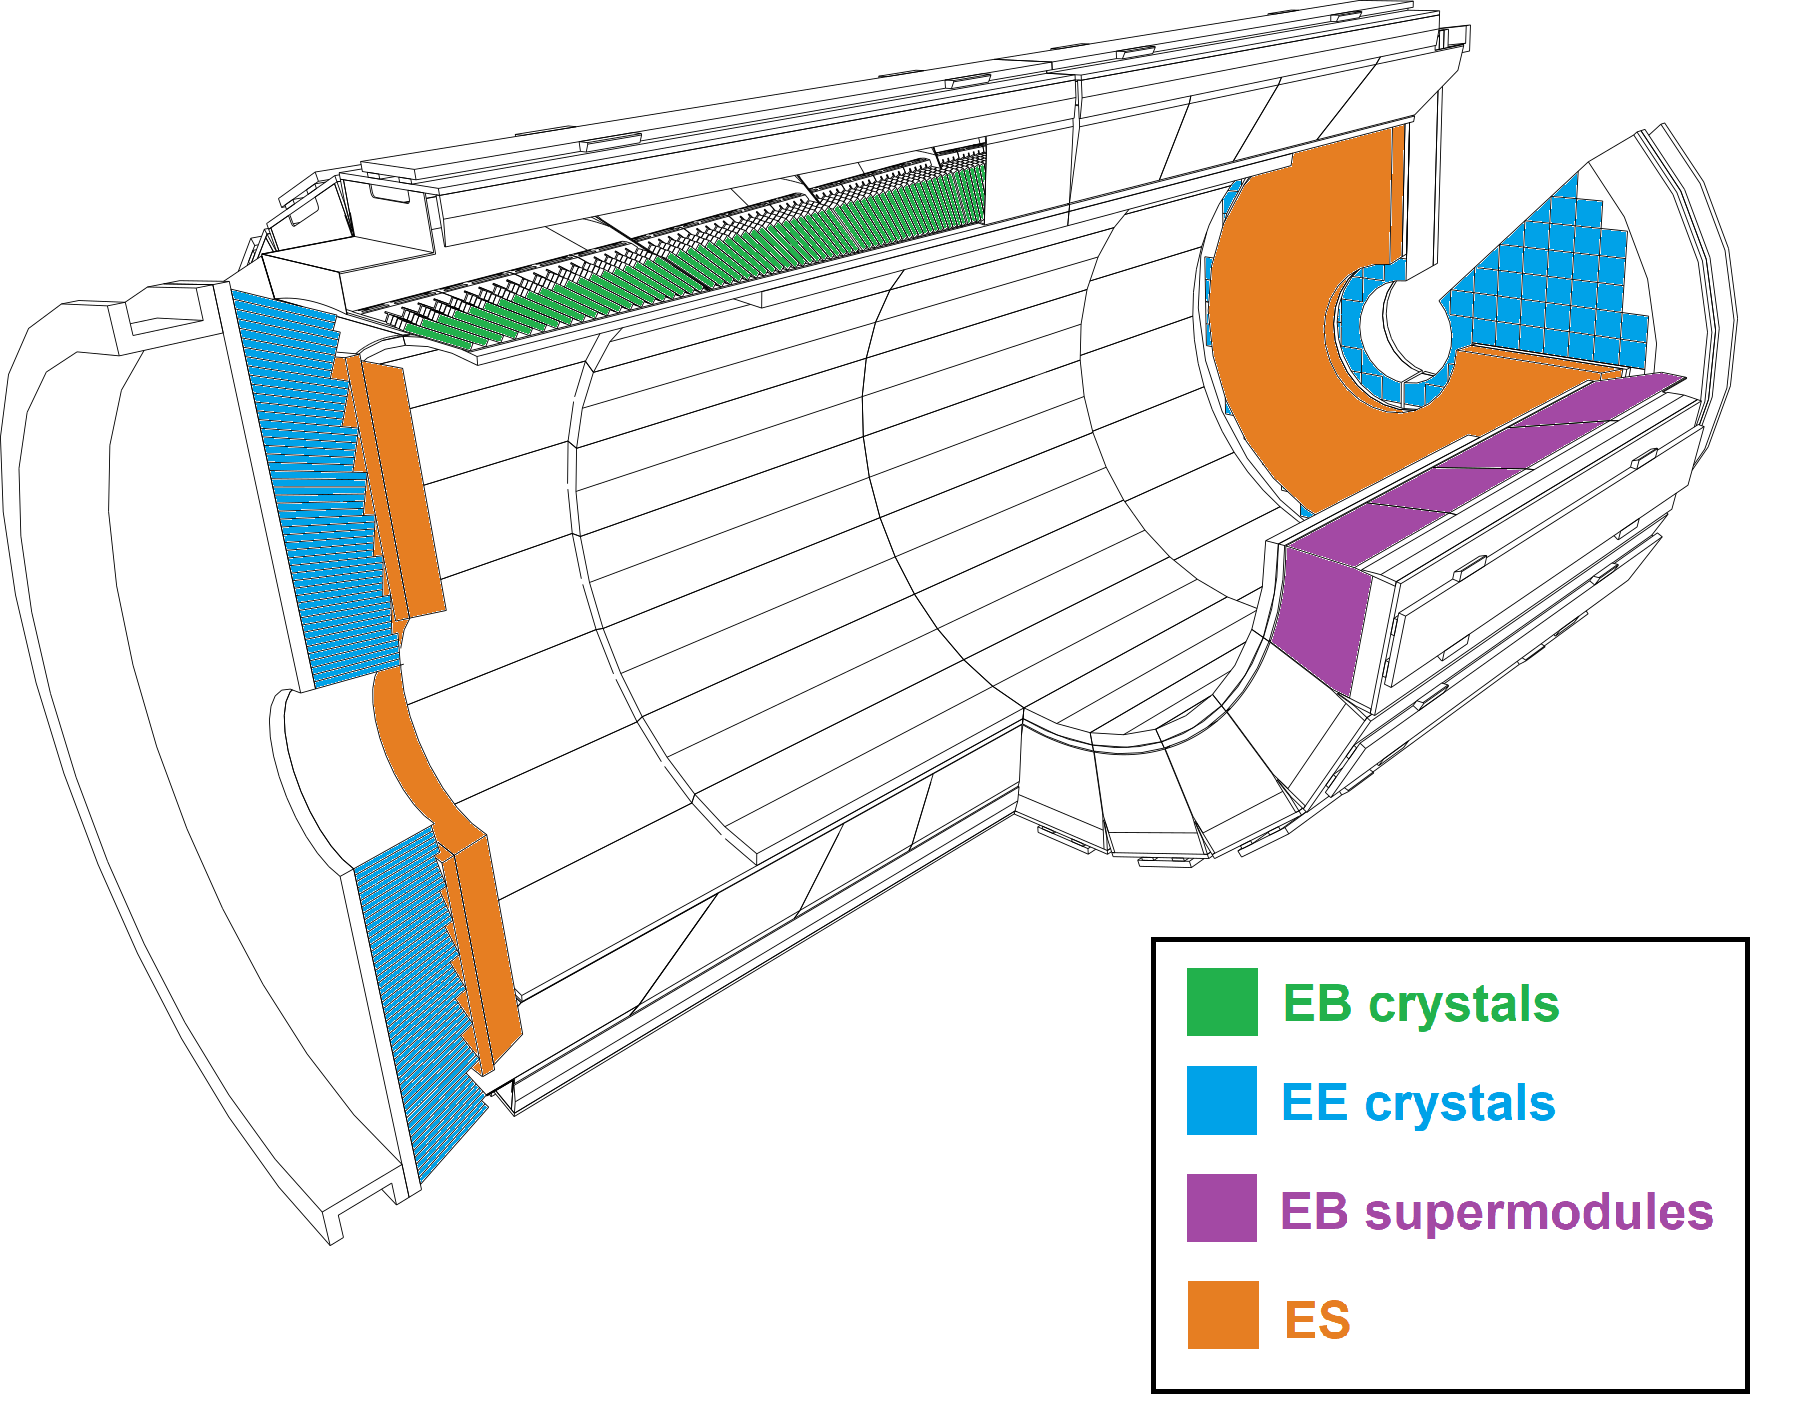
\includegraphics[width=0.65\textwidth]{Images/ECAL/Introduction/ECAL_ES_Diagram_colored.png}    
    \caption{CMS ECAL and ES partitions.}
    \label{fig:ECAL_Partitions}
\end{figure}

\begin{figure}[H]
    \centering
    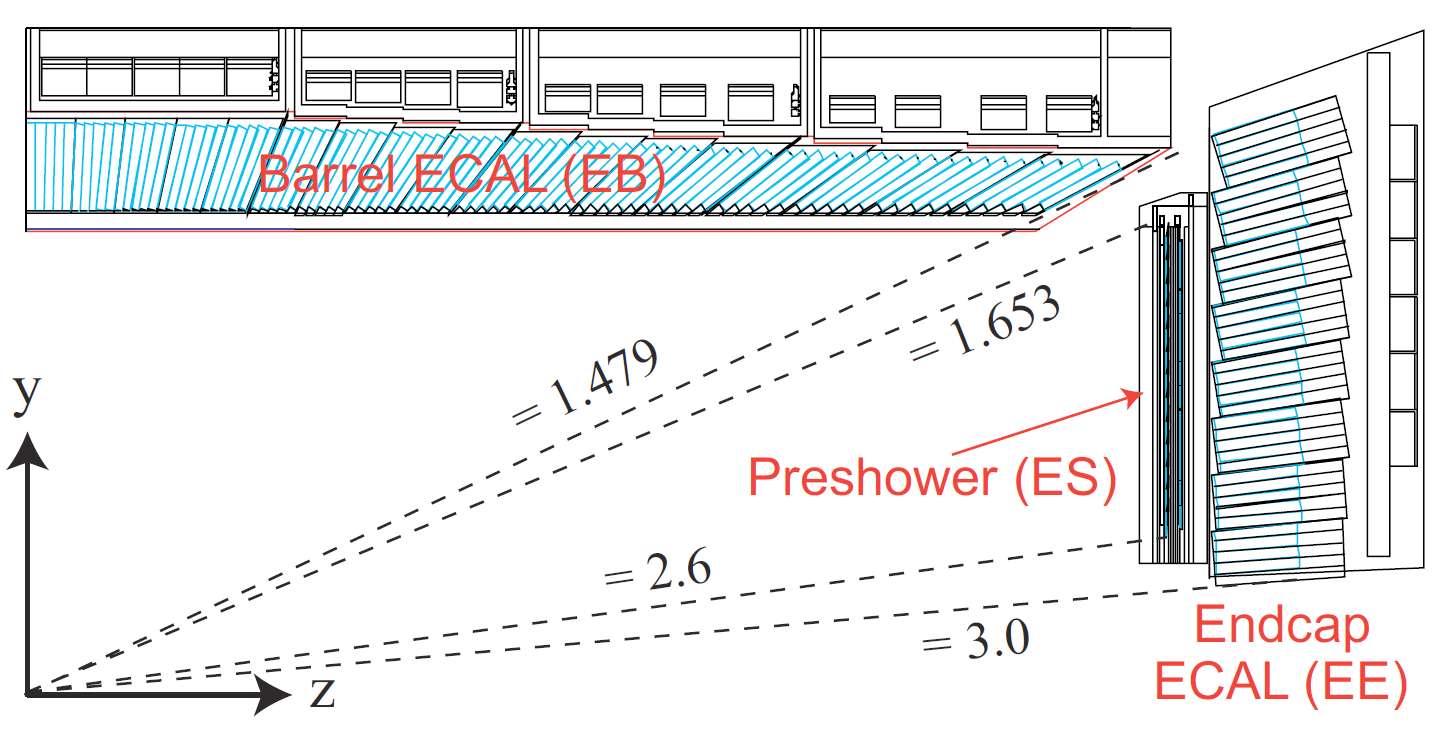
\includegraphics[width=0.65\textwidth]{Images/ECAL/Introduction/ECAL_Diagram.png}    
    \caption{Geometric coverage of the CMS ECAL and ES.}
    \label{fig:ECAL_Geometry}
\end{figure}

% https://cms.cern/detector/measuring-energy/ecal-preshower

\begin{figure}[H]%
    \setcounter{subfigure}{0}
    \centering
    \subfloat[ECAL barrel]{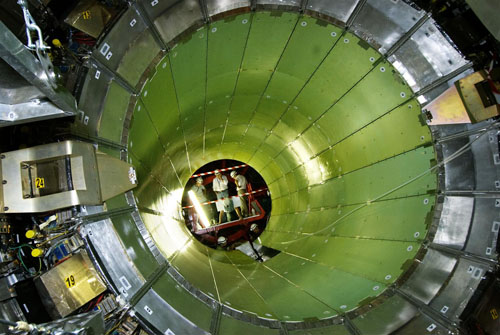
\includegraphics[width=.4\textwidth]{Images/ECAL/Introduction/EB_Image.jpg}}%
    \hfill
    \subfloat[Half of an ECAL endcap]{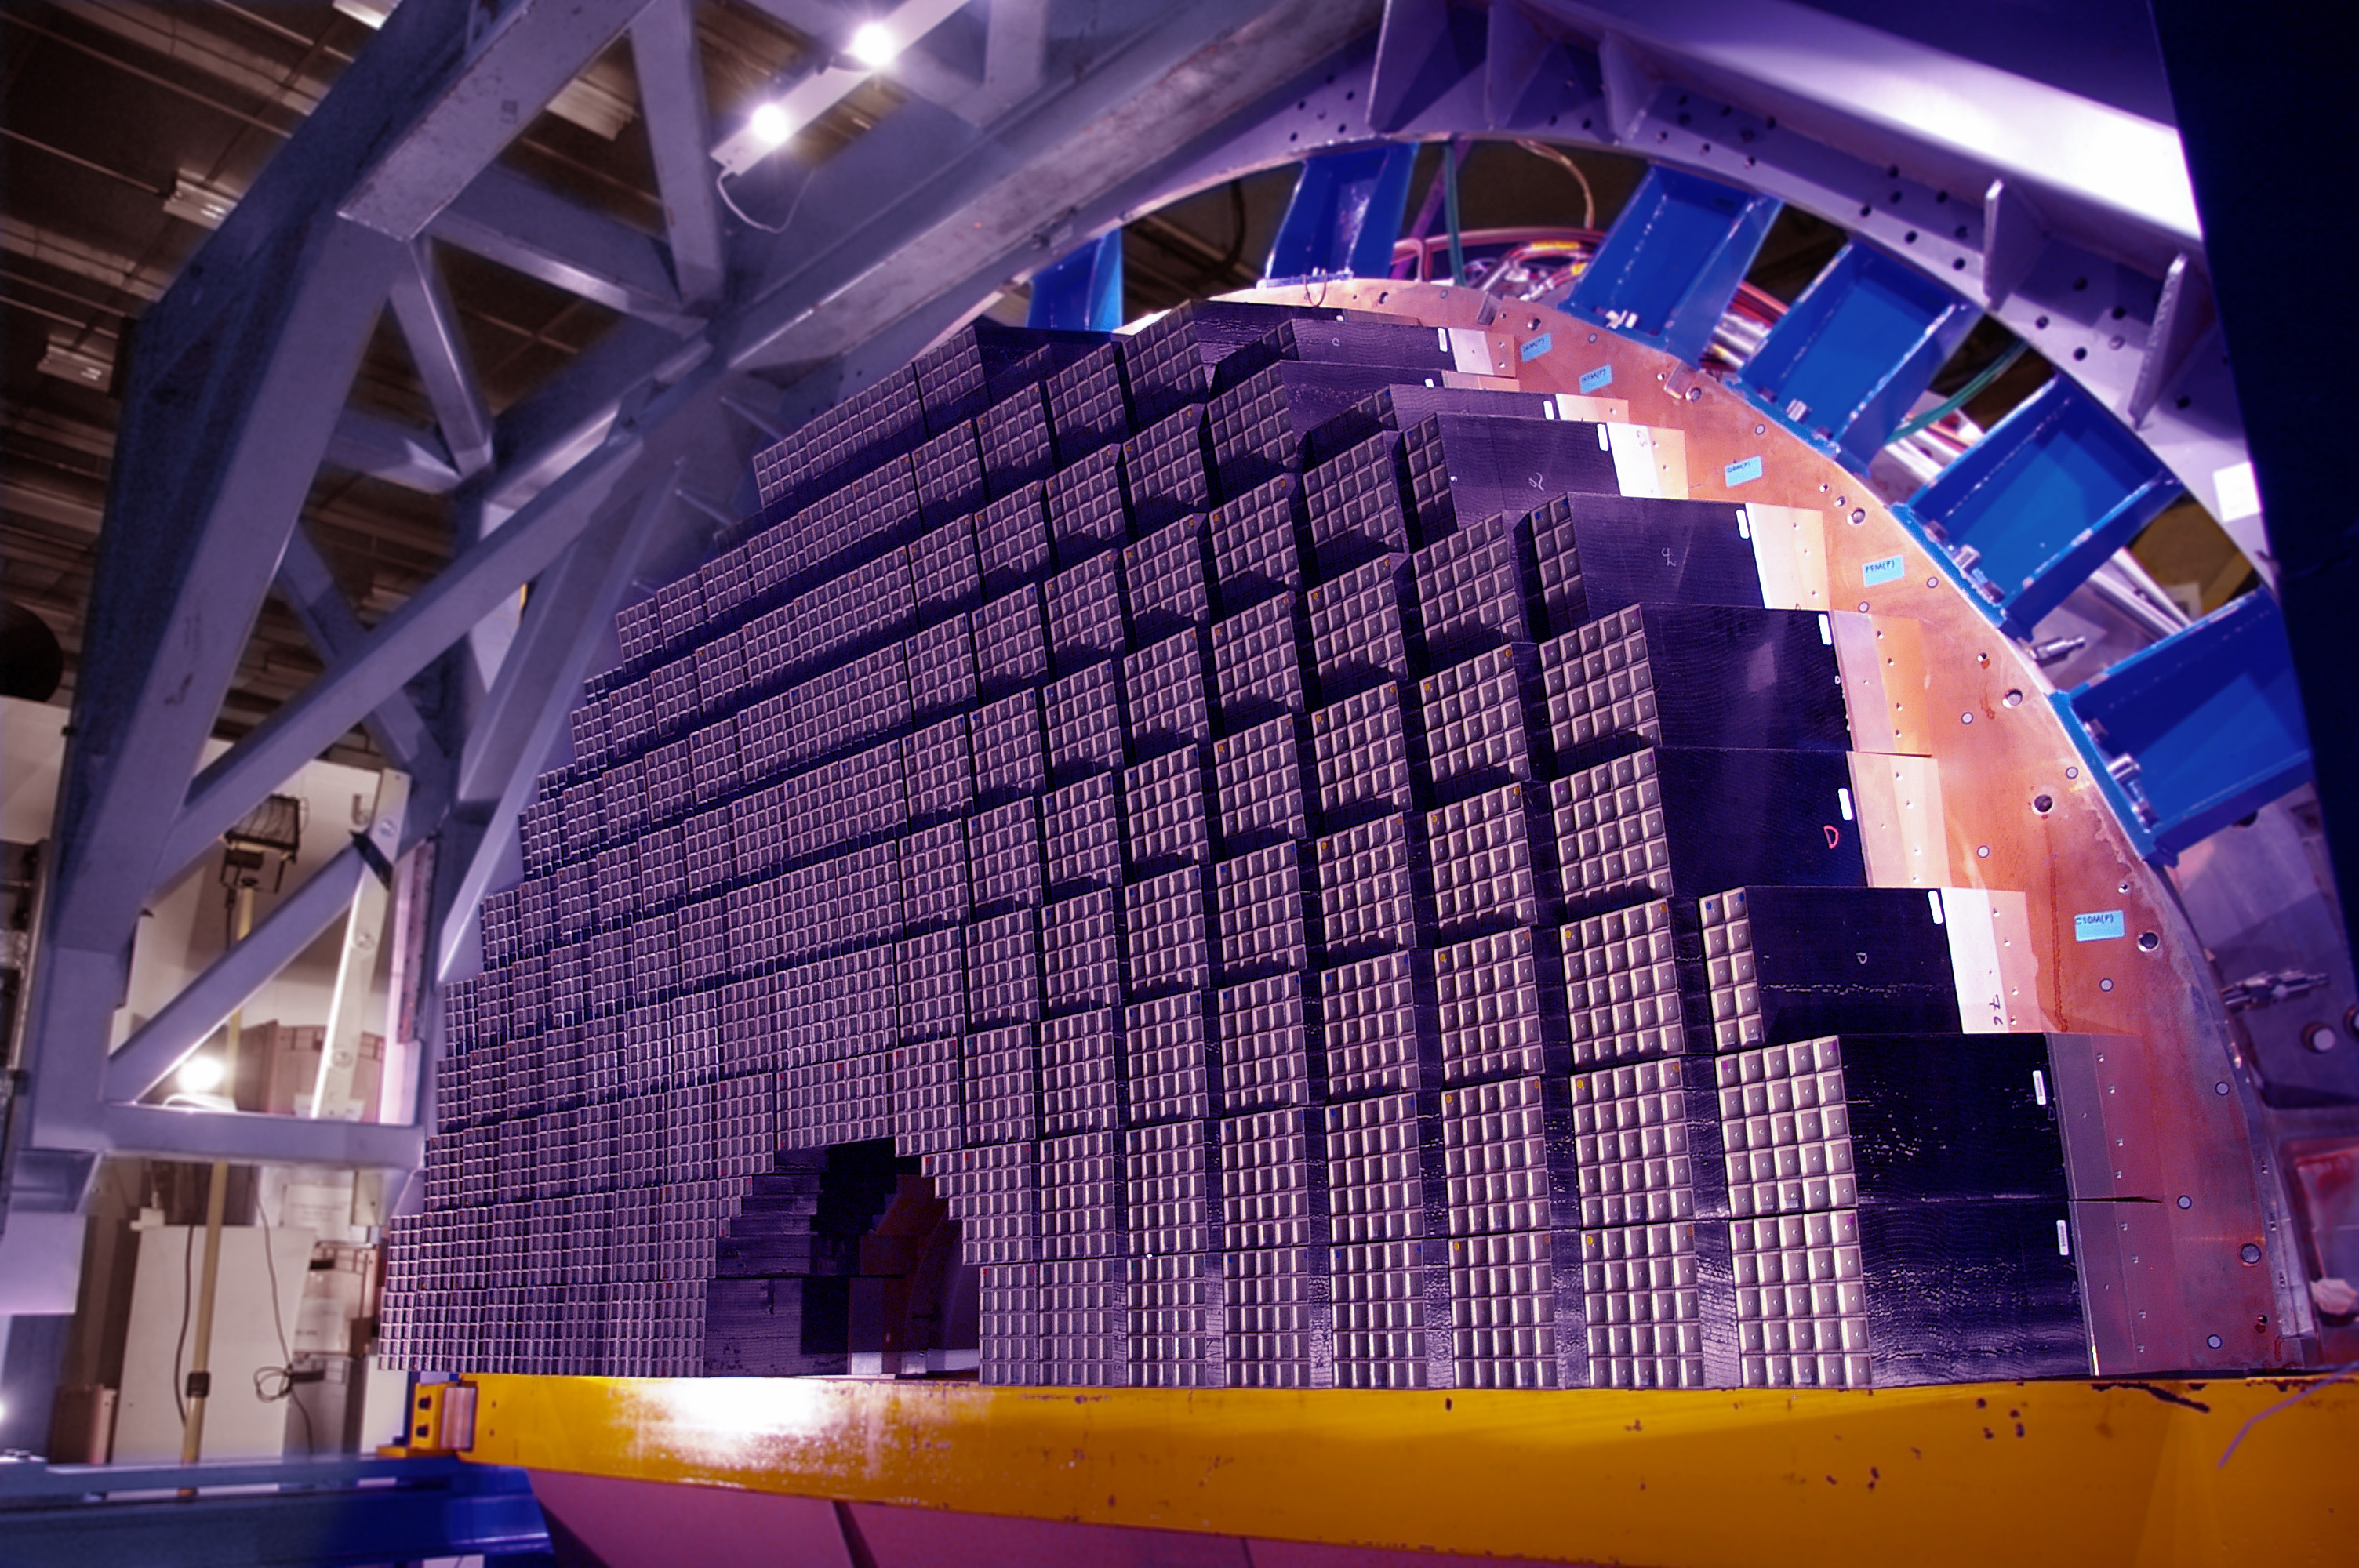
\includegraphics[width=.4\textwidth]{Images/ECAL/Introduction/EE_Half.jpg}}%
    \caption{Images of the CMS ECAL. \label{fig:ECAL_Images}}%
\end{figure}  

The basis of detection at ECAL is an electromagnetic shower. As a high energy electron or photon approaches ECAL, the electron will emit a photon as bremsstrahlung radiation, and the photon will pair produce to an electron-positron pair in the presence of massive detector material. The resulting photons, electrons, and positrons from this initial process will then perform the same types of processes as a cascade of particles is produced in the ECAL crystals. This is shown as a diagram in Fig. \ref{fig:Photon_Shower} for a photon initiating a shower, Fig. \ref{fig:Electron_Shower} for an electron initiating a shower, and is visualized as a simulation in Fig. \ref{fig:Simulated_Shower}. 

\begin{figure}[H]
    \centering
    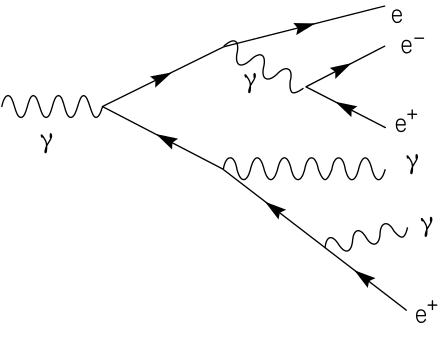
\includegraphics[width=0.7\textwidth]{Images/ECAL/Introduction/Photon_Shower.png}    
    \caption{Diagram form of a photon initiating an electromagnetic shower via pair production of an electron-positron pair.}
    \label{fig:Photon_Shower}
\end{figure}

\begin{figure}[H]
    \centering
    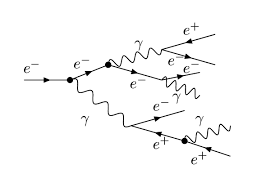
\includegraphics[width=0.7\textwidth]{Images/ECAL/Introduction/Electron_Shower.png}    
    \caption{Diagram form of an electron initiating an electromagnetic shower via bremsstrahlung radiation.}
    \label{fig:Electron_Shower}
\end{figure}

\begin{figure}[H]
    \centering
    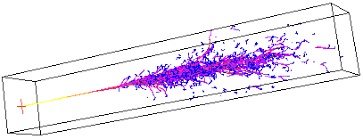
\includegraphics[width=0.7\textwidth]{Images/ECAL/Introduction/EM_Crystal_Shower.png}    
    \caption{Simulated electromagnetic shower inside a material.}
    \label{fig:Simulated_Shower}
\end{figure}

In ECAL, this EM shower leads to scintillation in its lead tungstate crystals, producing light that is read by photodetectors on the back of the crystals. The EB uses APDs (avalanche photodiodes), and the endcaps use VPTs (vacuum phototriodes) to convert scintillation light into an electrical signal. Digitized samples of ECAL are taken every 25 ns, and through a series of calibrations, the samples can be converted into an energy in GeV. An image of an EE crystal with its attached VPT is shown in Figure \ref{fig:ECAL_XTAL}.

% https://indico.cern.ch/event/1002959/contributions/4211462/attachments/2192922/3706736/EGM_Seminar_21-02-18.pdf

\begin{figure}[H]
    \centering
    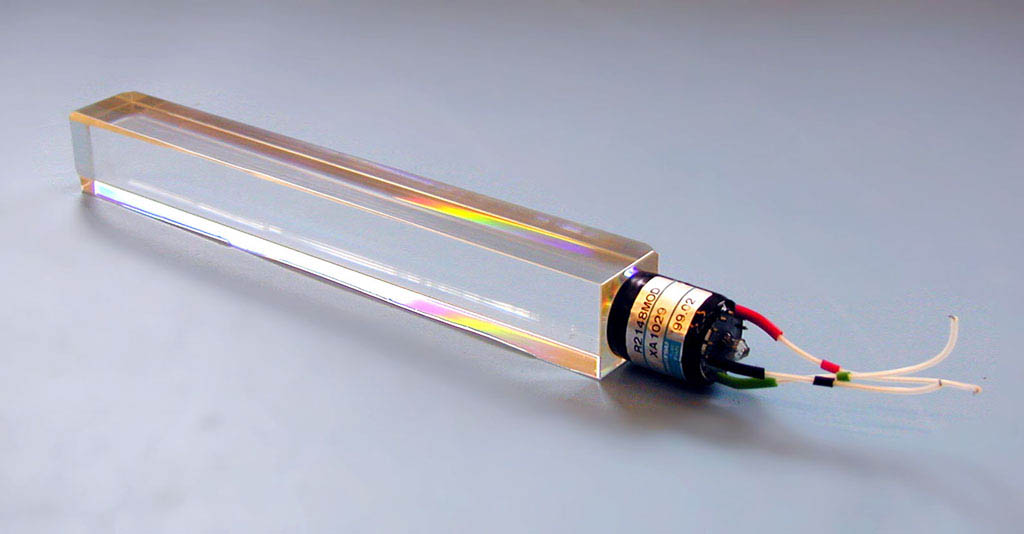
\includegraphics[width=0.7\textwidth]{Images/ECAL/Introduction/SC_VPT_and_crystal.jpg}    
    \caption{EE crystal with its attached VPT.}
    \label{fig:ECAL_XTAL}
\end{figure}